\chapter{Jednotlivé moduly ProtoPlantu}
ProtoPlant je modulární systém - není tedy jedním velkým celkem, se všemi funkcemi přímo zaintegrovanými.
V této kapitole se zaměřím na podrobný popis jednotlivých modulů.

\section{PPCU - ProtoPlant Control Unit}
PPCU, neboli řídící jednotka je hlavním modulem celého systému.
Samotné PPCU tvoří elektroinstalační box s krytím IP65.
Na přední části se nachází ovládací panel s LCD displejem a ovládacími tlačítky.
Z bočních stran jsou instalovány vodotěsné průchodky pro provlečení kabelů.

Uvnitř se nachází základní deska (viz. \autoref{subsec:motherBoard}) a zdroj napájení.

\section{Přídavné moduly ProtoPlantu}
Kromě samotné řídící elektroniky je možno ProtoPlant rozšířit i o přídavné moduly. 
Na vývoji těchto modulů se zatím stále pracuje.
Těchto modulů existuje hned několik:

\begin{itemize}
    \item CIPM (Communication Interface and Power Module  - modul potřebný pro drátové připojení ostatních modulů - viz. \autoref{subsec:CIPM})
    \item PSpl (Power Splitter - rozdělovač napájení)
    \item SHSM (Soil Humidity Sensorics Module - modul vybavený senzory pro měření vlhkosti půdy - viz. \autoref{subsec:SHSM})
    \item SEM (Sensorics Expansion Module - modul pro zvýšení počtu senzorů připojených k ProtoPlantu - viz. \autoref{subsec:SEM})
    \item PCM (Pump Control Module - modul pro sledování hladiny vody v nádrži a ovládání čerpadla - viz. \autoref{subsec:PCM})
    \item RCM (Remote Control Module - modul pro připojení vzdáleného ovládacího panelu - viz. \autoref{subsec:RCM})
\end{itemize}
Zjednodušené schéma zapojení a funkce jednotlivých modulů naleznete na \autoref{fig:add-MODULES}.

\paragraph{Napájení přídavných modulů}
je prováděno ve čtyřech režimech.
\begin{itemize}
    \item napájení přímo z řídící jednotky
    \item napájení z externího zdroje přes CIPM
    \item napájení přes PSpl
    \item napájení každého modulu odděleně
\end{itemize}

\subparagraph{Napájení přimo z řídící jednotky}
je možno použít pouze tehdy, když je připojen maximálně jeden modul a to z důvodu, aby bylo zabráněno podpětí celého systému.
Modul je takto připojen přímo k napájecímu okruhu A řídící jednotky (viz. \autoref{par:PowerCircuitA}).

\subparagraph{Použití externího zdroje připojeného k CIPM}
\label{subpar:suplyingViaCIPM}
je použitelné v případě, kdy uživatel upřednostňuje kabelovou komunikaci mezi moduly a řídící jednotkou.
Při napájení v tomto režimu je počet připojitelných modulů omezen pouze výkonem zdroje napájení připojeného k CIPM.
Na vstupní napájecí svorkovnici je připojen externí zdroj. 
Kromě dvou kabelů pro komunikaci jsou na výstupu připojeny i napájecí kabely od jednotlivých modulů.

\subparagraph{Napájení přes PSpl}
funguje na velmi podobném principu, jako předchozí varianta. 
K PSpl je na vstupní svorkovnici připojen externí zdroj napájení.
Na výstupních svorkovnicích jsou připojeny napájecí kabely jednotlivých modulů.
Tato metoda je určena primárně pro bezdrátovou komunikaci mezi řídící jednotkou a moduly.

\subparagraph{Napájení každého modulu odděleně}
je nejjednodušší metoda napájení.
Každý z modulů je připojen vlastním kabelem přímo k napájecímu zdroji.
Primárně je určena pro bezdrátovou komunikaci mezi jednotlivými moduly. 

\subsection{CIPM - Komunikační a napájecí modul}
\label{subsec:CIPM}
Tento modul funguje jako propojovací uzel mezi řídící jednotkou a všemi přídavnými moduly.
Dále slouží pro připojení externího napájení pro jednotlivé další moduly (viz. \autoref{subpar:suplyingViaCIPM}).

\subsection{SHSM - Modul měření vlhkosti půdy}
\label{subsec:SHSM}
Modul určený pro připojení senzorů měřících vlhkost půdy.
Tento modul je zatím stále ve stádiu konceptu.

\subsection{SEM - Modul rozšíření senzoriky}
\label{subsec:SEM}
Modul určený pro zvýšení pokrytí prostoru skleníku přidáním dalších enviromentálních senzorů.
Pro malé, případně středně velké skleníky není tento modul potřebný. 
Ve velkých sklenících již své uplatnění najde, vzhledem k tomu, že je vybaven vlastní řídící elektronikou a jediným omezením je dosah zvoleného způsobu komunikace s řídící jednotkou.

\subsection{PCM - Modul řízení čerpadel}
\label{subsec:PCM}
Valná většina zahrádkářů má pro svůj skleník i nádrž na vodu.
Tento modul je určen pro sledování hladiny vody v ní a případné spínání čerpadla, které má za úkol v nádrži vodu doplňovat.

\subsection{RCM - Modul vzdáleného ovládání}
\label{subsec:RCM}
Byl vytvořen pro zjednodušení nastavení a ovládání ProtoPlantu.
Skládá se ze dvou částí. 
Komunikační části, kterou lze připojit k základní desce ProtoPlantu a ovládacího panelu. 
Uživatel ovládací panel nainstaluje na zeď přímo v domě a může díky němu vzdáleně ovládat celý ProtoPlant přímo z pohodlí domova. 

\subsection{Uložení řídící elektroniky}
Řídící elektronika (základní deska, řadiče, kabeláž, atp.) je uložena v průmyslových elektroinstalačních boxech s krytím IP65 (\It{úplná prachotěsnost a odolnost proti tryskající vodě} \cite{IP_ratings}).
Vyvedení kabelů z těchto boxů je řešeno s pomocí kabelových průchodek se stejnou úrovní krytí.

Upevnění řídící elektroniky do těchto boxů je řešena díly vytisknutými na 3D tiskárně z materiálu ABS-T.
Ten jsem zvolil pro jeho odolnost a malou nasákavost.
Nevýhodou tohoto materiálu je nižší odolnost proti UV záření, proti kterému jsou ovšem díly v boxu chráněné.

Konstrukci pro upevnění tvoří zpravidla 3 části:
\begin{itemize}
    \item montážní deska
    \item kabelový unašeč
    \item kartuše se silikagelem
\end{itemize}

\noindent\B{Montážní deska} je největší částí celého držáku. 
Na spodní straně se nachází drážky pro správné umístění do boxu.
Z jedné z bočních stran se nachází drážky pro umístění kartuše se silikagelem.
Ze strany směřující do volného prostoru boxu se nacházejí výstupky, které se zasunou do drážek v montážní desce pro zdroj.
Na horní straně jsou umístěny otvory pro připevnění základní desky a drážky pro upevnění kabelových unašečů.

\noindent\B{Kabelové unašeče} jsou částí složenou z více menších dílů.
Jejich úkolem je upevnění kabelů do větších svazků pro vyšší přehlednost.

\noindent\B{Kartuše se silikagelem} má na sobě drážky pro zasunutí do jejich protikusů na montážní desce.

%\section{Ochrana elektroniky před přehřátím a vlhkostí}
%To be done.

\chapter{Tištěné spoje}
Všechny prototypy základních desek ProtoPlantu byly založeny na univerzálních tištěných spojích. Vzhledem k~tomu, že jsem po stránce vzhledu i funkčnosti nebyl s~takovýmto provedením spokojen, rozhodl jsem se nechat vyrobit vlastní tištěné spoje pro základní desku i senzorové moduly.
Díky tomuto jsem se naučil návrhu tištěných spojů a tvorbě výrobních podkladů v~programu Autodesk EAGLE.

\section{PPMB32 -- Základní deska}
\label{subsec:motherBoard}
Základní deska je rozdělena do několika částí. 
Vzhledem k~tomu, že umím pájet velmi dobře, rozhodl jsem se pro ruční osazení všech součástek, které byly doposud osazeny pouze na různých modulech připojených k~základní desce, včetně procesoru ESP32-WROOM32D.
Z~důvodu přehlednosti jsem desku rozdělil do několika částí:

\begin{itemize}
    \item Control (ESP32-WROOM32D a programátor)
    \item H-power (napájecí obvod a H-můstky)
    \item SIN (SensorIN - piny pro připojení senzorů)
    \item POUT (PowerOUT - výstup pro napájení dalších periferií)
    \item PanCon (PanelConnect - piny pro připojení tlačítek a displeje na ovládacím panelu)
    \item SelfProt (SelfProtection - senzor teploty a piny pro připojení vnitřního detektoru vody)
\end{itemize} 

Samotná základní deska má dvě verze. Jejich rozdíly jsou vysvětleny níže.
Obě verze desky jsou kromě sekce Control osazeny stejným hardwarem, tedy:

\begin{itemize}
    \item 2x H-můstek VNH2SP30
    \item regulátory napětí 7805CV-DG od STMicroelectronics
    \item pinheady pro připojení senzorů, ovládacího panelu a dalších periferií
    \item svorkovnicemi pro připojení napájecích kabelů a silových výstupů
\end{itemize}

Kromě dalších součástek je přímo na desce osazen senzor DS18B20 chránící desku před přehřátím. 
Pokud teplota základní desky překročí 50~\degree C, automaticky se přeruší veškeré operace a systém přejde do nouzového režimu (viz. kapitola \ref{paragraph:nouzovyRezim}).

\paragraph{PPMB32-F}
Kompletní, samostatná deska. 
Je přímo osazena procesorem ESP32-WROOM32D i programátorem CP2102N. 
Má nižší profil, tudíž je možné ji použít i v~menších prostorech.
Integrovaný programátor lze s~pomocí jumperů odpojit a přes programovací piny připojit externí. Tuto verzi jsem nazval PPMB32-F (označení F od anglického slova Full - kompletní).

\paragraph{PPMB32-E}
Vzhledem k~tomu, že je ProtoPlant veřejně dostupný, nebyl jsem si jist, zda by kompletní osazení takto velké desky zvládl i laik. 
Napadlo mě proto vytvořit i druhou desku, na které by byly osazeny dutinkové lišty pro vsazení vývojové ESP32 DevKitC. 
Odpadla by tedy nutnost kompletně osazovat sekci Control. 
Tuto verzi jsem nazval PPMB32-E (označení E od anglického slova Easy - jednoduchý).

\paragraph{Sekce Control}
Jak již bylo zmíněno, tato část desky zahrnuje modul procesoru ESP32-WROOM32D a programovací obvod. 
Ten se skládá z~převodníku USB-UART CP2102N, tranzistorů SS8050-G (sloužících pro reset procesoru), indikačních LED diod a mikro USB konektoru. 
Nachází se zde i jumper pro přepínání mezi externím programátorem a programátorem přímo na desce.

\paragraph{Sekce H-power}
V~této části desky se nacházejí H-můstky VNH2SP30 společně s~regulátory napětí 7805CV-DG (výstup 5VDC) a LM3940IT-3.3 (výstup 3,3VDC). 
Na verzi PPMB32-F je dále osazen AMS1117-3.3 pro napájení procesoru. 

V~dolní části desky se poté nacházejí dva integrované obvody VNH2SP30, z~nichž jeden (VNH1) je určen pro ovládání aktuátorů manipulujících s~okny a druhý 
(VNH2) má několik režimů funkce, podle připojeného výstupu:
\begin{itemize}
    \item disabled (výstupy jsou deaktivovány)
    \item pump (VNH je použito pro spínání čerpadla, případně stykače řídícího čerpadlo)
    \item heating (VNH je použito pro řízení topné spirály)
\end{itemize}

Napájení desky je rozděleno do tří okruhů. 

\paragraph{Okruh A}
\label{par:PowerCircuitA}
Tento okruh je určen pro napájení řídící elektroniky.
Má celkově 3 části, oddělené s~pomocí stabilizátorů napětí.
Jejich propojení znázorňuje schéma .

Rozsah vstupního napětí pro tento okruh je 7,5~VDC až 18~VDC.

\paragraph{Okruhy V1 a V2}
Použity pro oddělené napájení jednotlivých výstupů. 
Jejich napájecí rozsahy jsou rozepsány v~tabulce \ref{fig:powerSourceCharsVNH}.

\begin{table}[h]
    \centering
    \begin{tabular}{llll}
        \hline
        \multicolumn{1}{|l|}{\textbf{Parametr}}           & \multicolumn{1}{l|}{\textbf{Min.}} & \multicolumn{1}{l|}{\textbf{Max.}} & \multicolumn{1}{l|}{\textbf{Jednotka}} \\ \hline
        \multicolumn{1}{|l|}{Vstupní napětí}              & \multicolumn{1}{l|}{5,5}           & \multicolumn{1}{l|}{16}            & \multicolumn{1}{l|}{V}                 \\ \hline
        \multicolumn{1}{|l|}{Výstupní napětí}             & \multicolumn{1}{c|}{-}             & \multicolumn{1}{l|}{16}            & \multicolumn{1}{l|}{V}                 \\ \hline
        \multicolumn{1}{|l|}{Výstupní proud}              & \multicolumn{1}{c|}{-}             & \multicolumn{1}{l|}{30}            & \multicolumn{1}{l|}{A}                 \\ \hline
        \multicolumn{1}{|l|}{Maximální kontinuální proud} & \multicolumn{1}{c|}{-}             & \multicolumn{1}{l|}{14}            & \multicolumn{1}{l|}{A}                 \\ \hline
    \end{tabular}
    \caption{Tabulka napájecích rozsahů napájecích větví VNH1 a VNH2}
    \label{fig:powerSourceCharsVNH}
\end{table}

\paragraph{Sekce SIN}
Sekce s~piny pro připojení jednotlivých senzorů. 
S~výjimkou ochranných rezistorů je složena pouze z~pinheadů.
Jednotlivé piny jsou pro lepší přehlednost označeny přímo na desce a podrobněji popsány v~jejím datasheetu. 

\paragraph{Sekce POUT} 
Piny pro připojení napájení dalších periferií, modulů, či senzorů.
Je připojena k~napájecímu okruhu A.
Piny jsou rozděleny na části připojené k~subokruhům A1 a A2 s~napětím 3,3 a 5~VDC.

\paragraph{Sekce PanCon}
Dvanácti-pinový konektor PanCon slouží pro připojení kabelu od hlavního řídícího panelu. 
Samotný konektor má dva zemnící vývody, dva napájecí (1~x~5~V~a~1~x~3,3~V), dva vývody sběrnice I\textsuperscript{2}C a 6 vývodů pro připojení tlačítek a přepínačů.
Přesnější zapojení je opět k~dispozici v~datasheetech jednotlivých desek.

\section{PPSB - Desky se senzory teploty a vlhkosti}
Desky osazené senzory DS18B20\cite{DS18B20} (PPSB-T) a DHT22\cite{DHT22} (PPSB-TH).
Pro oba typy desek jsem navrhl a s pomocí 3D tisku vyrobil vlastní krabičky.\newline

\noindent\B{PPSB-T} -- deska osazená jedním senzorem DS18B20 \cite{DS18B20} zapojeným v režimu parazitního napájení (viz. \autoref{sec:DS18B20}).
V něm je senzor napájen přímo ze sběrnice OneWire, stačí mu tedy pro připojení pouze dva kabely (více v \cite{DS18B20}).
Deska má jednu vstupní a jednu výstupní stranu, senzory se takto dají řetězit.

Vizualizaci desky naleznete na obrázku \ref{fig:PPSB-T_VISUAL}.\newline \newline

\begin{figure}[h]
    \centering
   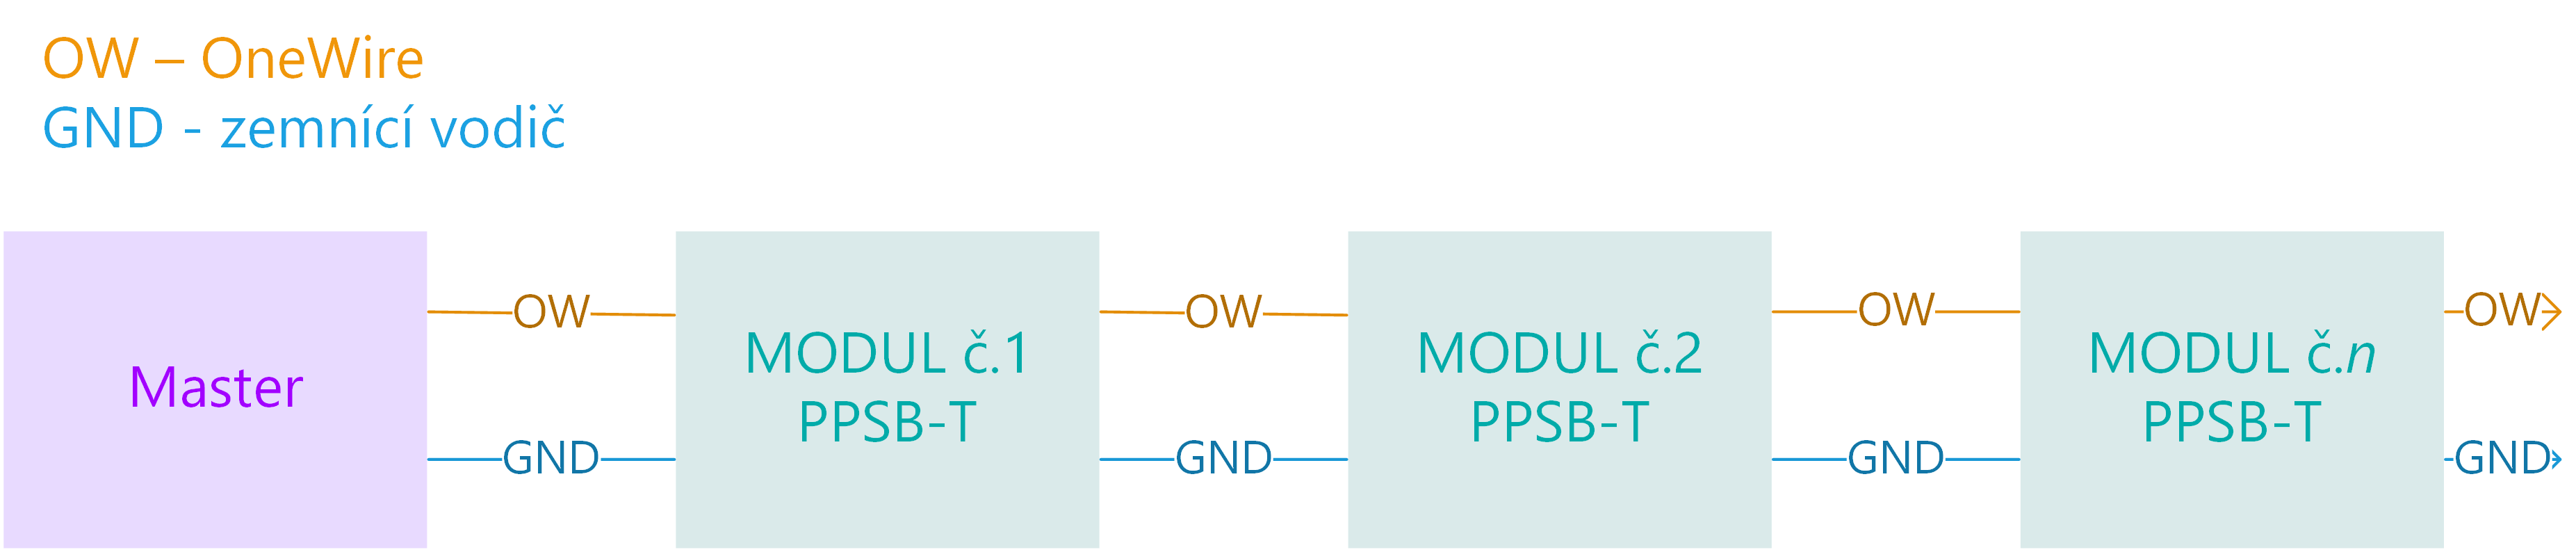
\includegraphics[width=\textwidth]{img/HARDWARE/PPSB-T_CHAIN.png}
   \caption{Řetězení desek PPSB-T.}
   \label{fig:PPSB-T_wiring}
\end{figure}

\noindent\B{PPSB-TH} osazena senzorem DHT22 \cite{DHT22} je schopna měřit vzdušnou vlhkost i teplotu.
Více o tomto senzoru naleznete v sekci \ref{sec:DHT22}.
Narozdíl od PPSB-T tyto desky nelze řetězit.
Vizualizace naleznete na obrázku \ref{fig:PPSB-TH_VISUAL}.\newline

\section{Senzorika}
ProtoPlant primárně podporuje 3 typy senzorů. 
DS18B20 pro měření teploty, BME280 schopné velmi přesně měřit vzdušnou vlhkost a DHT22 schopné měřit vlhkost i teplotu.
Dále ProtoPlant podporuje připojení senzorů vlhkosti půdy pracujících na bázi elektrické vodivosti.

\subsection{DS18B20}
\label{sec:DS18B20}
To be done.

\subsection{BME280}
\label{sec:BME280}
To be done.

\subsection{DHT22}
\label{sec:DHT22}
To be done.

\newpage